% %% %%%%%%%%%%%%%%%%%%%%%%%%%%%%%%%%%%%%%%%%%%%%%%%%%%%%%%%%%%
% step-2.tex
%
% Author:  Mauricio Matamoros
% License: MIT
%
% %% %%%%%%%%%%%%%%%%%%%%%%%%%%%%%%%%%%%%%%%%%%%%%%%%%%%%%%%%%%

%!TEX root = ../practica.tex
%!TEX root = ../references.bib

% CHKTEX-FILE 1
% CHKTEX-FILE 8
% CHKTEX-FILE 13
% CHKTEX-FILE 46

\subsection{Paso 2: Configuración con buildroot}%
\label{sec:step2}
Para generar un kernel optimizado se utilizará \emph{buildroot}.
Buildroot permite no sólo configurar y compilar un kernel Linux personalizado, sino la imagen del sistema completo incluyendo el sistema de archivos con los programas embebidos y cualesquiera paquetes necesarios para ejecutarlos.


\subsubsection*{Paso 2.1. Descarga y descompresión}

El primer paso consiste en descargar buildroot de \url{https://buildroot.org/download.html}, por ejemplo mediante la línea:

\begin{Verbatim}[gobble=1]
	$ wget https://buildroot.org/downloads/buildroot-2025.02.tar.xz
\end{Verbatim}

\noindent
A continuacíón descomprima buildroot en la carpeta de su proyecto, por ejemplo con:

\begin{Verbatim}[gobble=1]
	$ tar xf buildroot-2025.02.tar.xz
\end{Verbatim}

\noindent
e ingrese al directorio, por ejemplo \texttt{cd buildroot-2025.02}.

El siguiente paso consiste en verificar que tenemos todos los paquetes necesarios para el proyecto dentro de \emph{buildroot}.
Verifique que \texttt{python-smbus2} está disponible ejecutando el comando \texttt{ls package/python-* | grep smbus2}.
Debería ver una salida como la siguiente:
\begin{Verbatim}[gobble=1]
	$ ls package/python-* | grep smbus2
	package/python-smbus2:
	python-smbus2.hash
	python-smbus2.mk
\end{Verbatim}

Si estos archivos no estuvieren disponibles, será necesario crearlos.
El prodecimiento para crear dichos archivos se detalla en el \Cref{sec:add-smbus2}.




\subsubsection*{Paso 2.2. Selección de arquitectura objetivo}

\emph{buildroot} permite la creación de imágenes de Linux para prácticamente cualquier arquitectura soportada.
La lista de configuraciones incluidas se puede obtener con el comando \texttt{make list-defconfigs} cuya salida puede ser un poco larga, por lo que la recortaremos con \texttt{grep}, obteniendo una salida como la siguiente:

\begin{Verbatim}[gobble=1]
	$ make list-defconfigs | grep raspberry
	    raspberrypi0_defconfig              - Build for raspberrypi0
	    raspberrypi0w_defconfig             - Build for raspberrypi0w
	    raspberrypi2_defconfig              - Build for raspberrypi2
	    raspberrypi3_64_defconfig           - Build for raspberrypi3_64
	    raspberrypi3_defconfig              - Build for raspberrypi3
	    raspberrypi3_qt5we_defconfig        - Build for raspberrypi3_qt5we
	    raspberrypi4_64_defconfig           - Build for raspberrypi4_64
	    raspberrypi4_defconfig              - Build for raspberrypi4
	    raspberrypicm4io_64_defconfig       - Build for raspberrypicm4io_64
	    raspberrypicm4io_defconfig          - Build for raspberrypicm4io
	    raspberrypi_defconfig               - Build for raspberrypi
	    raspberrypizero2w_defconfig         - Build for raspberrypizero2w
\end{Verbatim}

El siguiente paso consiste en seleccionar la configuración base para la arquitectura a generar.
En nuestro caso tomaremos como base una Raspberry Pi 4 con sistema de 64 bits.
\begin{Verbatim}[gobble=1]
	$ make raspberrypi4_64_defconfig
\end{Verbatim}




\subsubsection*{Paso 2.2. Configuración del sistema}
Invoque interfaz de buildroot con el comando

\begin{Verbatim}[gobble=1]
	$ make menuconfig
\end{Verbatim}

\noindent verá una pantalla similar a la de la \Cref{fig:mc-main}.

\begin{figure}[H]
	\centering
	\begin{subfigure}[b]{0.5\textwidth}
		\centering
		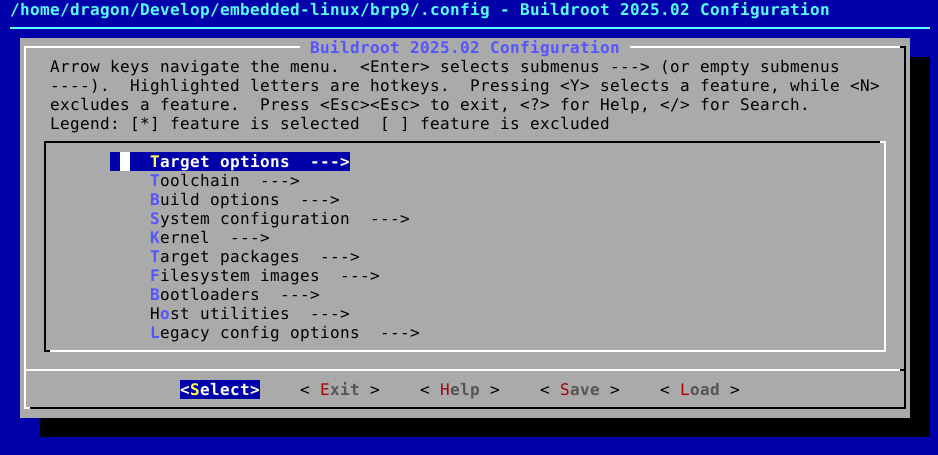
\includegraphics[width=0.95\textwidth,height=5cm,keepaspectratio]{img/make-mc-main.png}
		\caption{Menú principal}%
		\label{fig:mc-main}
	\end{subfigure}%
	\begin{subfigure}[b]{0.5\textwidth}
		\centering
		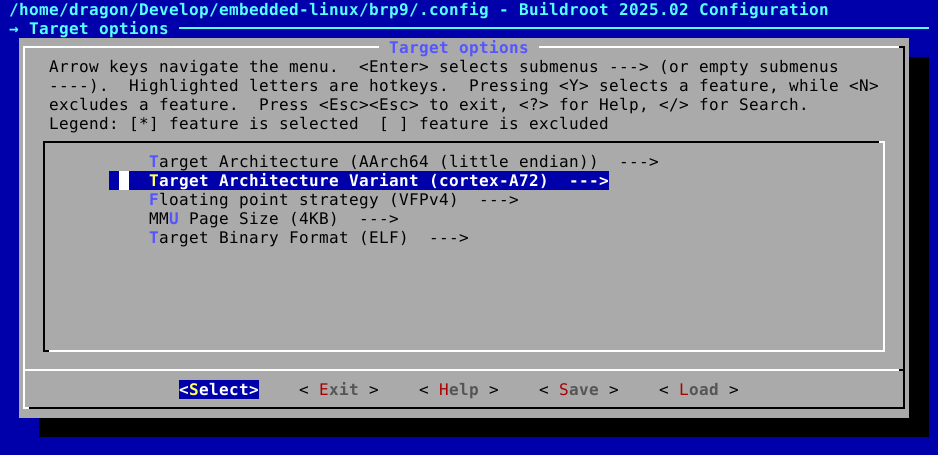
\includegraphics[width=0.95\textwidth,height=5cm,keepaspectratio]{img/make-mc-target.png}
		\caption{Arquitectura objetivo (menú \emph{target options})}%
		\label{fig:mc-target}
	\end{subfigure}\\
	\begin{subfigure}[b]{0.5\textwidth}
		\centering
		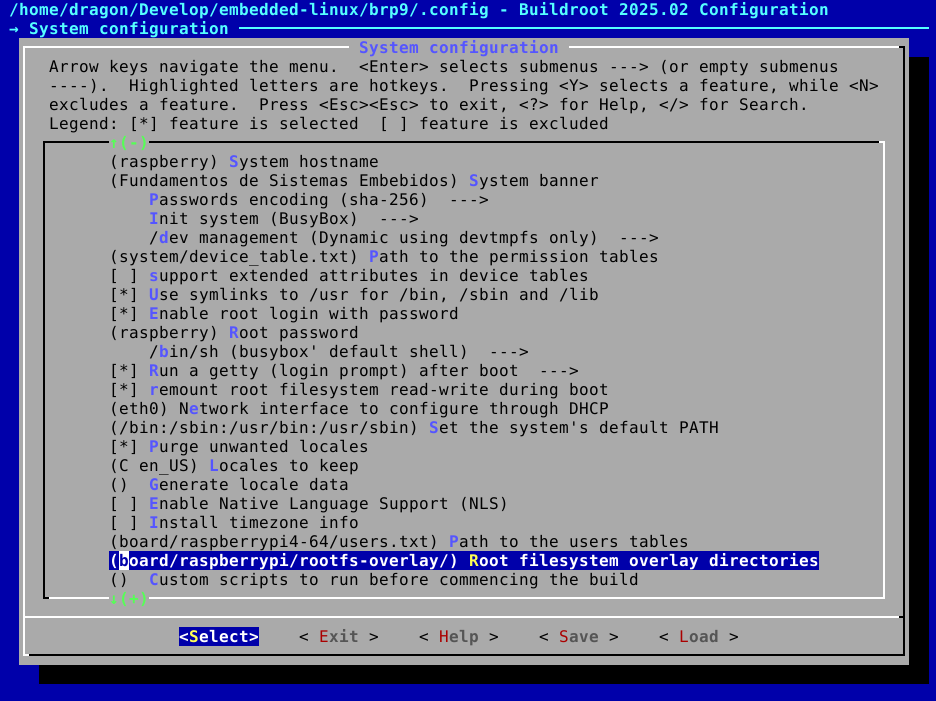
\includegraphics[width=0.95\textwidth,height=7cm,keepaspectratio]{img/make-mc-sysconfig.png}
		\caption{Configuración del sistema (menú \emph{system configuration})}%
		\label{fig:mc-sysconfig}
	\end{subfigure}%
	\begin{subfigure}[b]{0.5\textwidth}
		\centering
		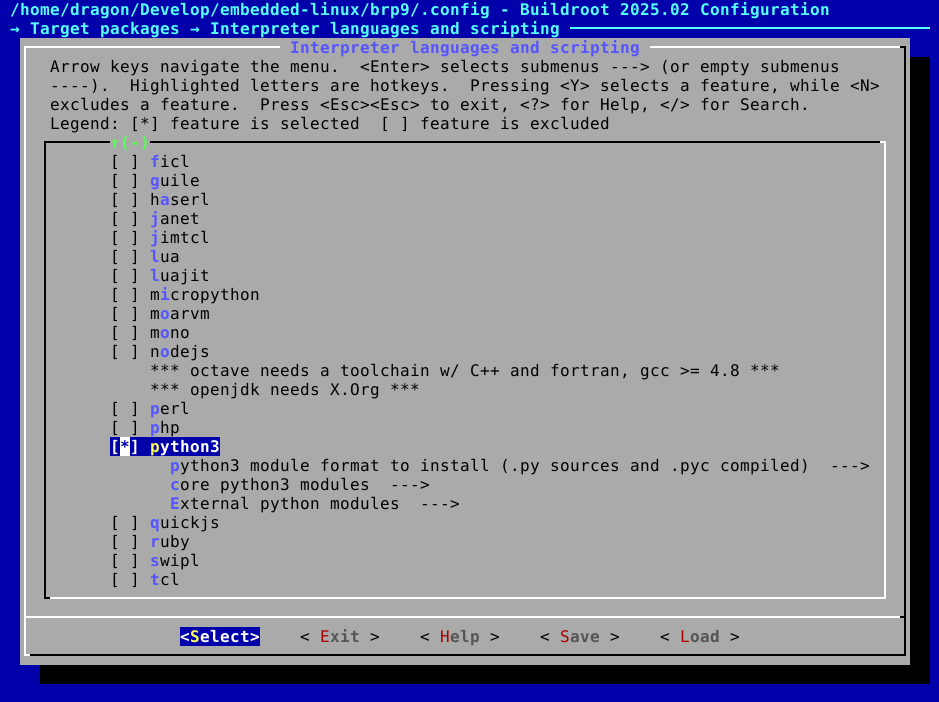
\includegraphics[width=0.95\textwidth,height=7cm,keepaspectratio]{img/make-mc-python3.png}
		\caption{Paquete \texttt{python3} habilitado (menú \emph{target packages})}%
		\label{fig:mc-python3}
	\end{subfigure}
	\caption{Interfaz gráfica de buildroot (modo consola)}%
	\label{fig:make-menuconfig}
\end{figure}

A continuación, tómese unos minutos para familiarizarse con el entorno gráfico.
En particular revise el \texttt{toolchain} y el \texttt{target}.
En este último notará que la arquitectura es \texttt{AArch64} para el cortex-A72
tal como se muestra en la~\Cref{fig:mc-target}.

Bajo \emph{Build Options} se cambiarán tres valores.
El primero es establecer \emph{Location to save buildroot config} con el valor \texttt{./.config} para evitar sobreescribir la configuración predeterminada.
El segundo es \emph{global patch and hash directories} con el valor \texttt{board/raspberrypi4-64/patches}; directorio en el cual se copiarán los parches que se aplicarán al Kernel previo a la compilación del mismo y que será usado en el siguiente paso (véase~\Cref{sec:step3}).
El tercer y último valor es habilitar la compilación de librerías para que éstas estén disponibles tanto en su versión dinámica como estática; cambiando \emph{libraries} a \texttt{both}.

En el menú de configuración del sistema (\emph{System Configuration}) se definirán siete valores:
\begin{enumerate*}[label=\alph*\rpar]
	\item el nombre del sistema (\emph{system hostname}) se establece a {raspberry}, aunque se recomienda que los estudiantes utilicen el nombre de la brigada o equipo;
	\item el saludo inicial o estandarte(\emph{system banner}) que se establece al nombre de la asignatura,
	\item la habilitación de los directorios
		\texttt{/bin},
		\texttt{/sbin} y
		\texttt{/lib}
		como enlaces simbólicos dentro de \texttt{/usr};
	\item la habilitación del usuario de root para iniciar sesión (\emph{enable root login})
	y, por consiguiente,
	\item establecer la contraseña de root (\emph{root password}) a \texttt{raspberry}.
	\item Por último, se establece el path de la tabla de usuarios (\emph{path to the users tables})
	y
	\item el directorio que contendrá el sistema de archivos raíz (\emph{root filesystem overlay directories}).
\end{enumerate*}
Se presenta un resúmen de estos valores en la \Cref{tbl:menuconfig-changes}.

\medskip{}

\begin{importantbox}{Advertencia de seguridad}
	Habilitar el inicio de sesión para el súper usuario \emph{root} es una tremenda falla de seguridad ya que permite a los usuarios malintencionados tomar control del sistema.
	Se habilita en esta práctica para permitir al estudiante depurar su código \emph{in situ}.

	Los sistemas en producción deberán deshabilitar esta opción.
\end{importantbox}



\subsubsection*{Paso 2.3. Selección de paquetes preinstalados}

El siguiente paso es crítico, ya que es aquí donde se habilitará el intérprete de python con todas sus librerías, así como cualquier programa necesario.
Dentro del menú de paquetes objetivo (\emph{target packages}) ubique el sub-menú de lenguajes interpretados y de scripting (\emph{interpreter languages and scripting})
Dentro de éste localice \texttt{python3} y habilítelo.

De manera automática se actualizará el menú mostrando nuevas opciones bajo la recién habilitada \texttt{python3}.
El primer cambio importante consiste en cambiar el módulo de soporte de formatos a instalar (\emph{python3 module format to install}).
De forma predeterminada buildroot instala soporte sólo para archivos de python precompilados \texttt{pyc};
un tipo de archivo que contiene código en bytes similar a los formatos de Java y C\# que pueden ser interpretados por Python sin exponer el código fuente del mismo.
Sin embargo, estos archivos tienen el inconveniente de que deben ser generados para una versión específica del intérprete.
Por este motivo es conveniente para el estudiante habilitar el soporte de archivos de scripting \texttt{.py}.

Los siguientes dos menús contienen la lista de módulos de python disponibles para embebir.
Nuestro sistema embebido no estará configurado para conectarse a internet ni incluye un gestor de paquetes, por lo que no se podrá usar ni \texttt{apt} ni \texttt{pip3} para instalar paquetes.
Estos tendrán que venir ya incluidos y compilados para nuestros sistema.

Navegue dentro del menú de modulos externos de Python (\emph{external python modules}) y habilite los paquetes \texttt{python-pigpio} y \texttt{python-smbus2} que agregó previamente al inicio de esta sección.

\medskip{}

De forma similar a como habilitó \texttt{python3}, ubique el submenú de componentes de hardware (Hardware handling) dentro del menú de paquetes objetivo (\emph{target packages})
y habilite las herramientas para \IIC{} que aparecen como \texttt{i2c-tools}.

\begin{table}
	\caption{Lista de cambios a realizar en \texttt{make menuconfig}}
	\label{tbl:menuconfig-changes}
	\centering
	\begin{tabularx}{\columnwidth}{X l}
	\toprule
	\multicolumn{1}{c}{\textbf{Submenú}}                   &
	\multicolumn{1}{c}{\textbf{Valor}} \\
	\midrule
		Build Options → Location to save buildroot config & \texttt{./.config} \\
		Build Options → libraries                         & \texttt{both} \\
		Build Options → global patch and hash directories & \texttt{board/raspberrypi4-64/patches} \\[2mm]

		System Configuration → System hostname            & \texttt{raspberry} \\
		System Configuration → System banner              & \texttt{Fundamentos de Sistemas Embebidos} \\
		System Configuration → Use symlinks\dots{}        & \texttt{y} \\
		System Configuration → Enable root login          & \texttt{y} \\
		System Configuration → Root password              & \texttt{raspberry} \\
		System Configuration → Path to the users tables   & \texttt{board/raspberrypi4-64/users.txt} \\
		System Configuration → RootFS overlay directories & \texttt{board/raspberrypi4-64/rootfs-overlay/} \\[2mm]

		Kernel → Custom boot logo file path               & \texttt{board/raspberrypi4-64/logo.png} \\[2mm]

		Target packages → Interpreter languages and scripting → \\
		~~~~python3                                       & \texttt{y} \\
		~~~~python3 → python3 module format to install    & \texttt{.py sources and .pyc compiled} \\
		~~~~python3 → External python modules → \\
		~~~~~~~~\texttt{python-pigpio}                    & \texttt{y} \\
		~~~~~~~~\texttt{python-smbus2}                    & \texttt{y} \\[2mm]
		Target packages → Hardware handling →             \\
		~~~~i2c-tools                                     & \texttt{y} \\

		Filesystem images → exact size                    & \texttt{250M} \\[2mm]
	\bottomrule
	\end{tabularx}
\end{table}


\subsubsection*{Paso 2.4. Configuraciones finales de la imagen}

El siguiente paso consiste en reservar suficiente espacio en la imagen para el proyecto.
Navegue al menú imágenes del sistema de archivos (\emph{filesystem images}) localizado en la pantalla principal y cambie el el tamaño exacto de la imagen (\emph{exact size}) a \texttt{250M} como se muestra en la~\Cref{tbl:menuconfig-changes}.

Finalmente, tras cerrar \texttt{menuconfig}, es necesario habilitar en el kernel la carga de los controladores \IIC{}.
Para este propósito, edite el archivo \texttt{config.txt} de su modelo de raspbery en el directorio correspondiente.
En nuestro caso (una Raspberry Pi 4 con sistema operativo de 64 bits) es el archivo \texttt{board/raspberrypi4-64/config\_4\_64bit.txt}.
Agregue las siguientes líneas al final:

\begin{Verbatim}[gobble=1]
	# Enable kernel drivers for i2c1
	dtparam=i2c1=on
\end{Verbatim}

O bien, puede simplemente ejecutar esta línea:

\begin{Verbatim}[gobble=1]
	$ echo -e "# enable i2c\ndtparam=i2c1=on" >> board/raspberrypi4-64/config_4_64bit.txt
\end{Verbatim}

De forma similar, es necesario agregar un usuario con privilegios limitados (por seguridad no queremos que los programas se ejecuten con privilegios elevados).
Esto se logra proporcionando a \emph{buildroot} un archivo con la tabla de usuarios con sus grupos, directorios y permisos.
Para este fin crearemos el archivo \texttt{board/raspberrypi4-64/users.txt} con el siguiente texto:

\begin{minipage}{\columnwidth}
\lstinputlisting[%
	title={\texttt{board/raspberrypi4-64/users.txt}},%
	firstnumber=1%
]{src/board/raspberrypi4-64/users.txt}
\end{minipage}
